\subsection{Aplicación web}

Para realizar pruebas unitarias a la aplicación web desarrollado con Django se utilizo la herramienta que permite analizar que partes del código de un programa se están ejecutando y con ello determinar que bloques de código se deben de someter a pruebas.

Al utilizar coverage.py sobre el proyecto de Django se obtuvieron los resultados que se muestran en la figura \ref{fig:coverage}. El reporte que coverage.py arroja muestra la cantidad de código que se tiene que probar, el código que falta por probar, el excluido y el que se tienen cubierto con las pruebas.

Se logro cubrir el 100\% del código y se excluyeron algunas partes debido a que forman parte de los archivos de configuración de Django y porque fueron pruebas complicadas de elaborar.

\begin{figure}[H]
	\centering
	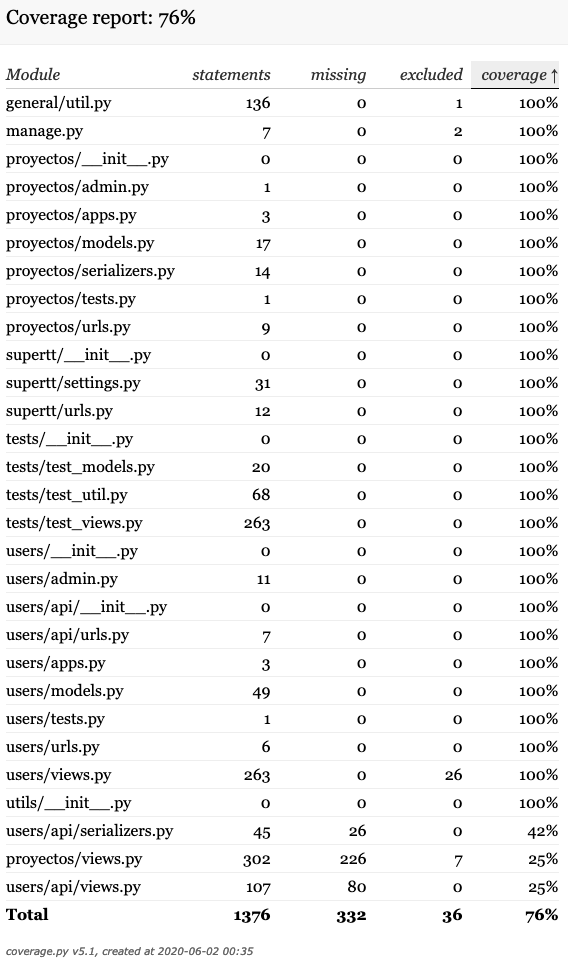
\includegraphics[width=250px]{capitulo6/unitarias/img/coverage.png}
	\caption{Reporte del código sometido a pruebas}
	\label{fig:coverage}
\end{figure}

Para realizar pruebas sobre estos bloques de código encontrados, se utilizo el módulo de pruebas unitarias con el que cuenta Django y se realizaron pruebas sobre los modelos, vistas y las clases de utilitaria que se desarrollaron.

Como se puede apreciar en la figura \ref{fig:pruebasDjango}, se realizaron 777 pruebas sobre modelos, vistas y utilitaria, al final siendo exitosas cada una de ellas.

\begin{figure}[H]
	\centering
	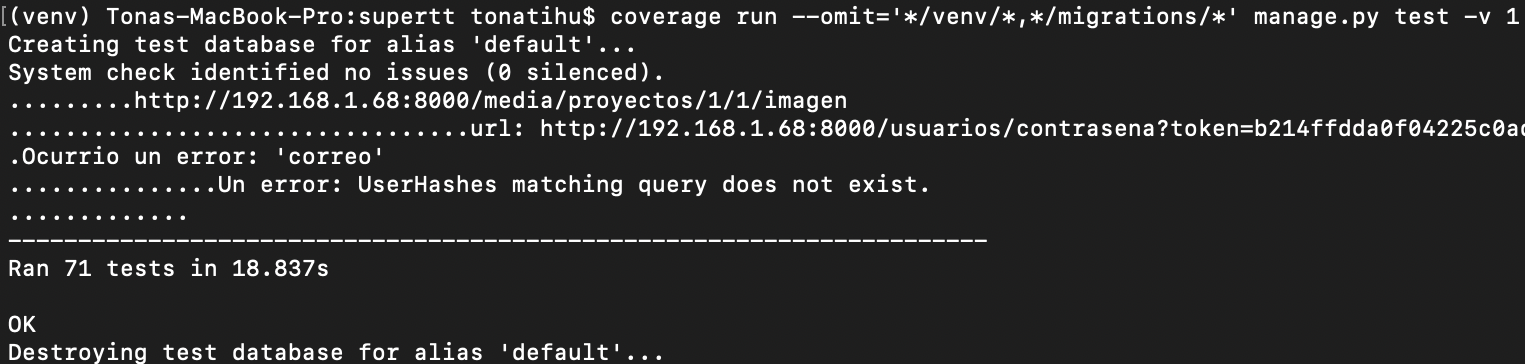
\includegraphics[width=450px]{capitulo6/unitarias/img/pruebasDjango.png}
	\caption{Resultado de las pruebas de Django}
	\label{fig:pruebasDjango}
\end{figure}

La forma en la que se elaboraron estas pruebas fue la siguiente.

\subsubsection{Pruebas sobre los modelos}

Un ejemplo de las pruebas sobre modelos es el siguiente código, en el cual se prueba el modelo del usuario y en cada uno de los métodos que comienzan con la palabra test determinan los diferentes casos de prueba a elaborar, que en este ejemplo son sobre el guardado de información de un usuario.

\lstinputlisting[language=Python]{capitulo6/unitarias/codigo/test_models.py}

En las primeras dos pruebas se utiliza el método assertEquals el cual permite comparar el resultado de una prueba con el esperado para determinar si la prueba fue exitosa.

Para las siguientes tres pruebas como se espera que se arroje una excepción se utiliza la declaración with para determinar si la excepción esperada ocurrió y con ello asegurar que la prueba fue exitosa, si esto no ocurre la prueba no es correcta. 

\subsubsection{Pruebas sobre los vistas}

\lstinputlisting[language=Python]{capitulo6/unitarias/codigo/test_views.py}

\subsubsection{Pruebas sobre las clases de utilitaria}

\lstinputlisting[language=Python]{capitulo6/unitarias/codigo/test_util.py}
